\documentclass{jarticle}
\usepackage[dvipdfmx]{graphicx}
\usepackage{here}
\usepackage{listings,jlisting}


\lstset{
  basicstyle={\ttfamily},
  identifierstyle={\small},
  commentstyle={\smallitshape},
  keywordstyle={\small\bfseries},
  ndkeywordstyle={\small},
  stringstyle={\small\ttfamily},
  frame={tb},
  breaklines=true,
  columns=[l]{fullflexible},
  numbers=left,
  xrightmargin=0zw,
  xleftmargin=3zw,
  numberstyle={\scriptsize},
  stepnumber=1,
  numbersep=1zw,
  lineskip=-0.5ex
}

\title{{システム実験}\\実験9回レポート}
\author{6119019056 山口力也}
\date{2019/06/21日提出}

\begin{document}
\maketitle
\section{LPFの効果と伝達関数}
\subsection{目的}
課題5.1の目的は何か?100文字以上で答えよ. \\

課題5.1ではロータリエンコーダの量子化誤差などが1次のLPFを通して観測値を平滑化することによってどのように軽減されるかグラフを作成してわかりやすく理解した.さらに表示したグラフからゲインと時定数を読み取り,モータの伝達関数を推定した.伝達関数を推定した後は,Scilabによるシミュレーションを行った.このシミュレーションが出力フィルタ値とほぼ同じ値を取り,大まかな動きをとらえていることを確認することでシミュレーションが有効なことを確認した.

\subsection{実験結果}
課題5.1の結果を報告せよ.その際,モータの回転速度,duty比などのデータをScilabを用いてグラフにすること. \\

以下図\ref{fig:kadai5-1-1}にモータの回転速度と時間のグラフを示す.

\begin{figure}[H]
\begin{center}
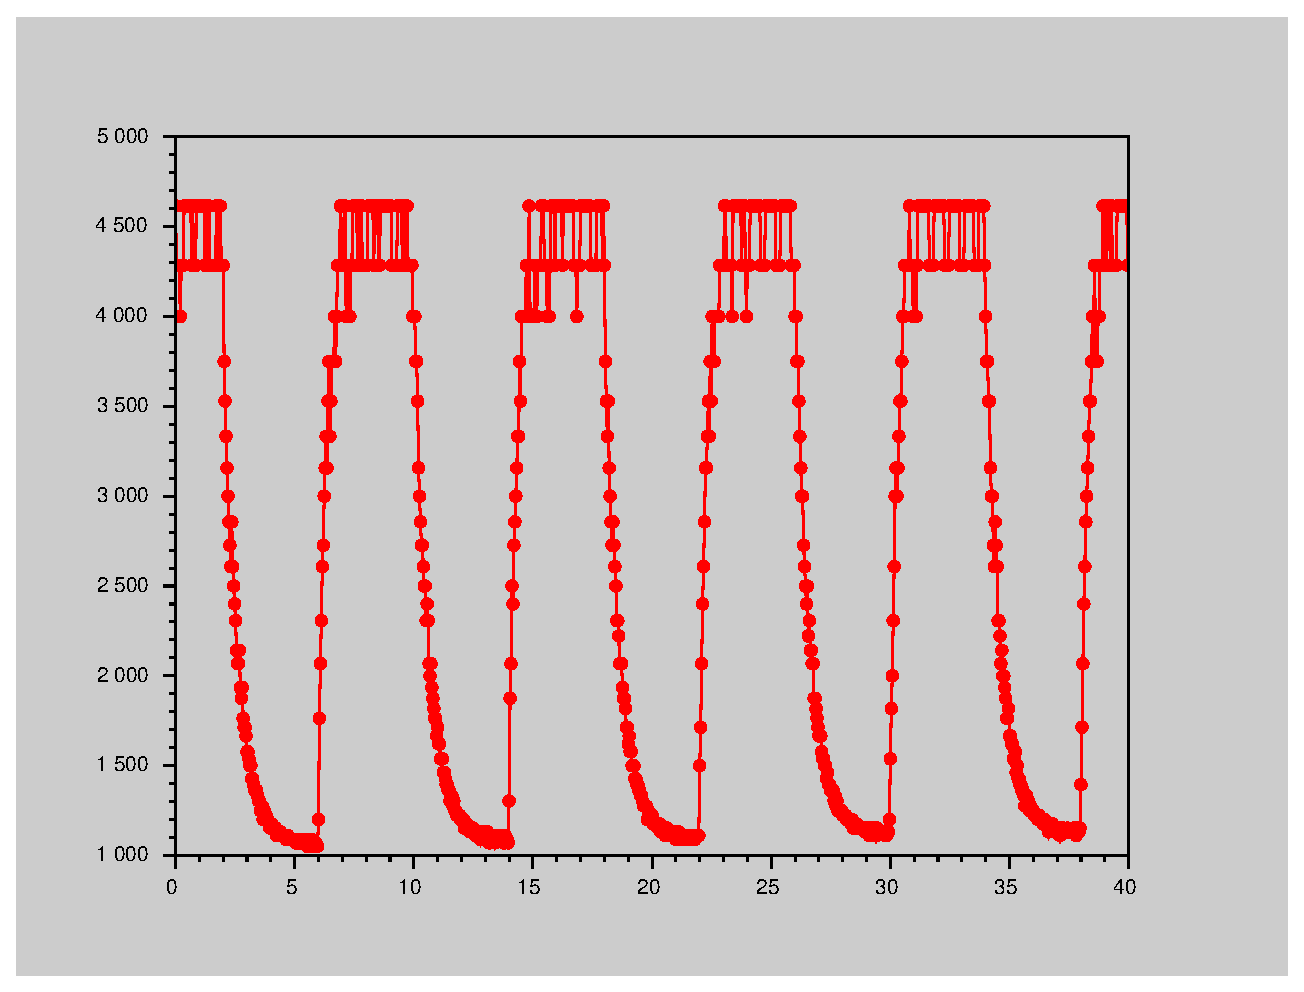
\includegraphics[width=7.0cm]{images/kadai5-1-1.eps}
\caption{課題5.1の出力画像(平滑化なし)}
\label{fig:kadai5-1-1}
\end{center}
\end{figure}

以下図\ref{fig:kadai5-1-2}にduty比と時間のグラフを示す.

\begin{figure}[H]
\begin{center}
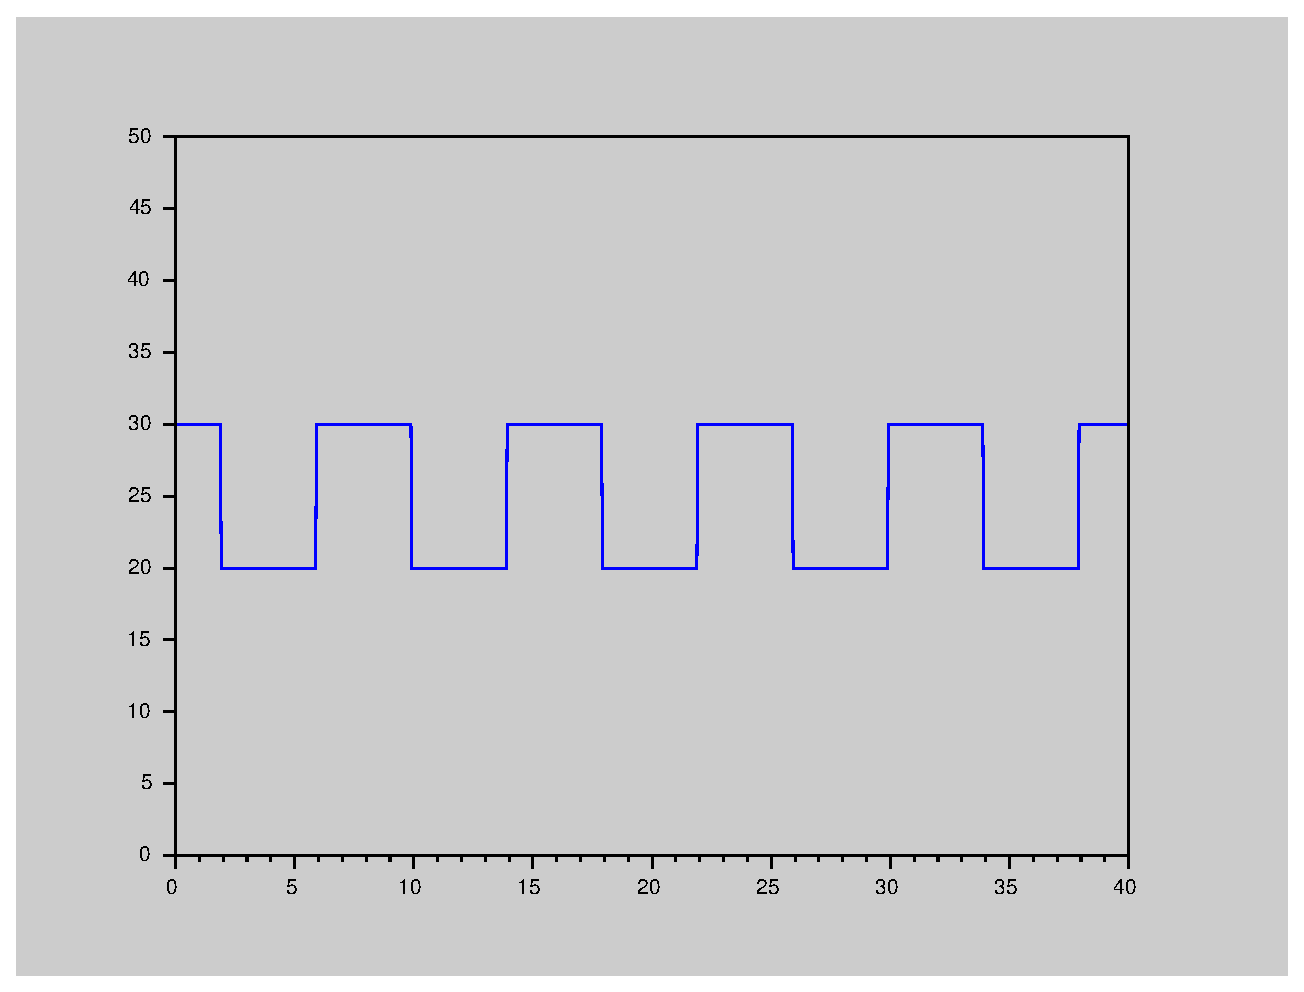
\includegraphics[width=7.0cm]{images/kadai5-1-2.eps}
\caption{課題5.1の出力画像(duty比)}
\label{fig:kadai5-1-2}
\end{center}
\end{figure}


以下図\ref{fig:kadai5-1-3}にLPFを通し平滑化した後のモータの回転速度と時間のグラフを示す.

\begin{figure}[H]
\begin{center}
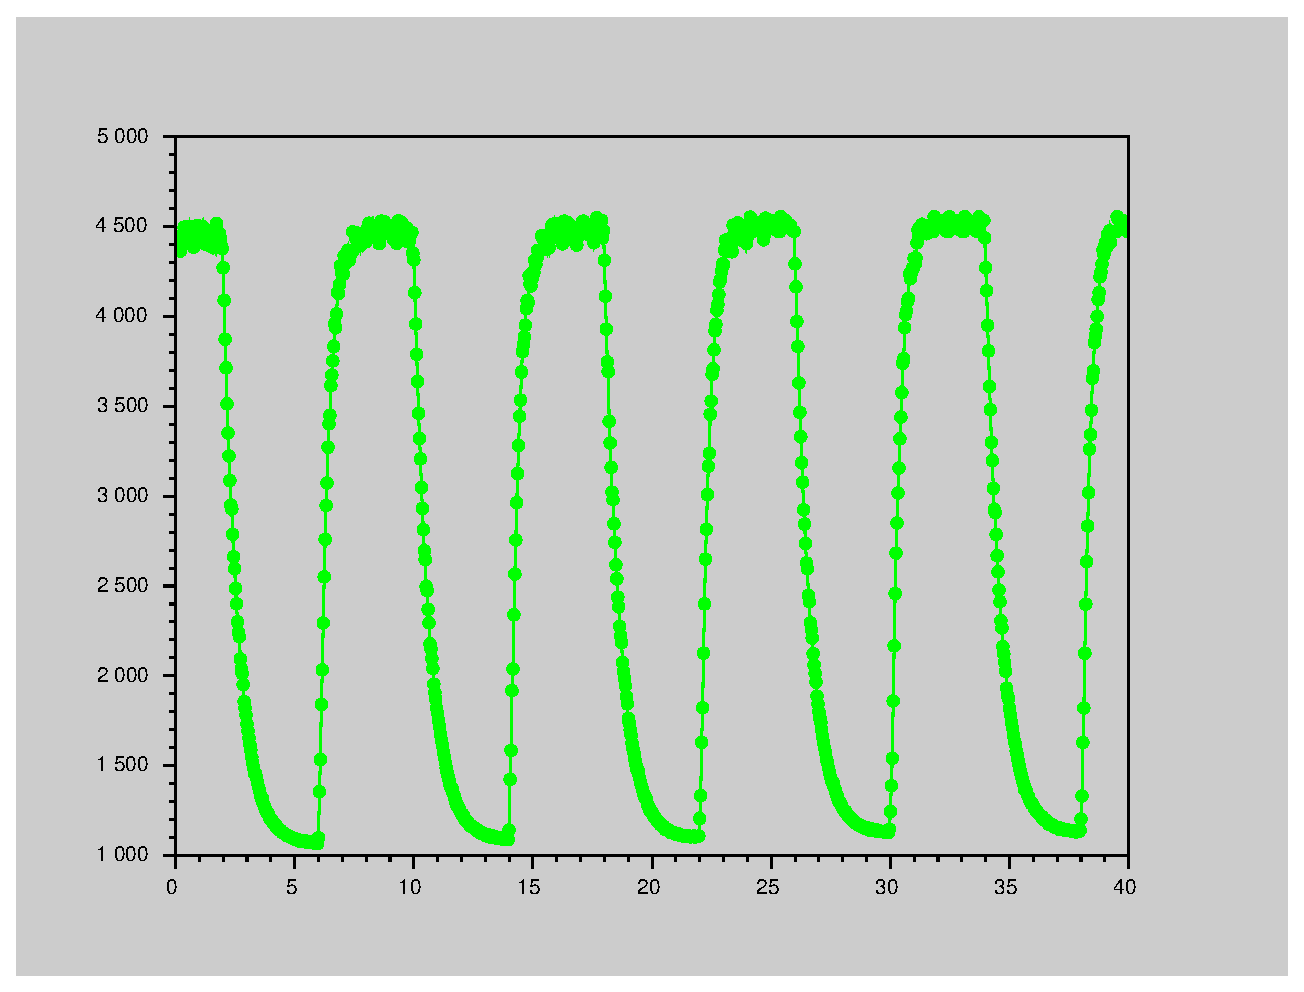
\includegraphics[width=7.0cm]{images/kadai5-1-3.eps}
\caption{課題5.1の出力画像(平滑化)}
\label{fig:kadai5-1-3}
\end{center}
\end{figure}

\subsection{平滑化の結果}
平滑化処理の有無でどのような違いがみられたか報告せよ. \\

平滑化処理を入れることで,雑音が大幅に軽減された.これは信号の周波数帯域は低周波から高周波まで広く分布しているのに対して,雑音は比較的高周波帯域に分布しているためだと考えられる.

\subsection{伝達関数の推定}
制御入力(duty比)とモータの回転速度の関係から,モータの時定数と定常ゲインを読み取り,対象の伝達関数を求めよ.また,読み取りに使用した拡大グラフを貼り付けよ. \\

以下図\ref{fig:kadai5-1-3-expand}に読み取りに使用した拡大グラフを示す.

\begin{figure}[H]
\begin{center}
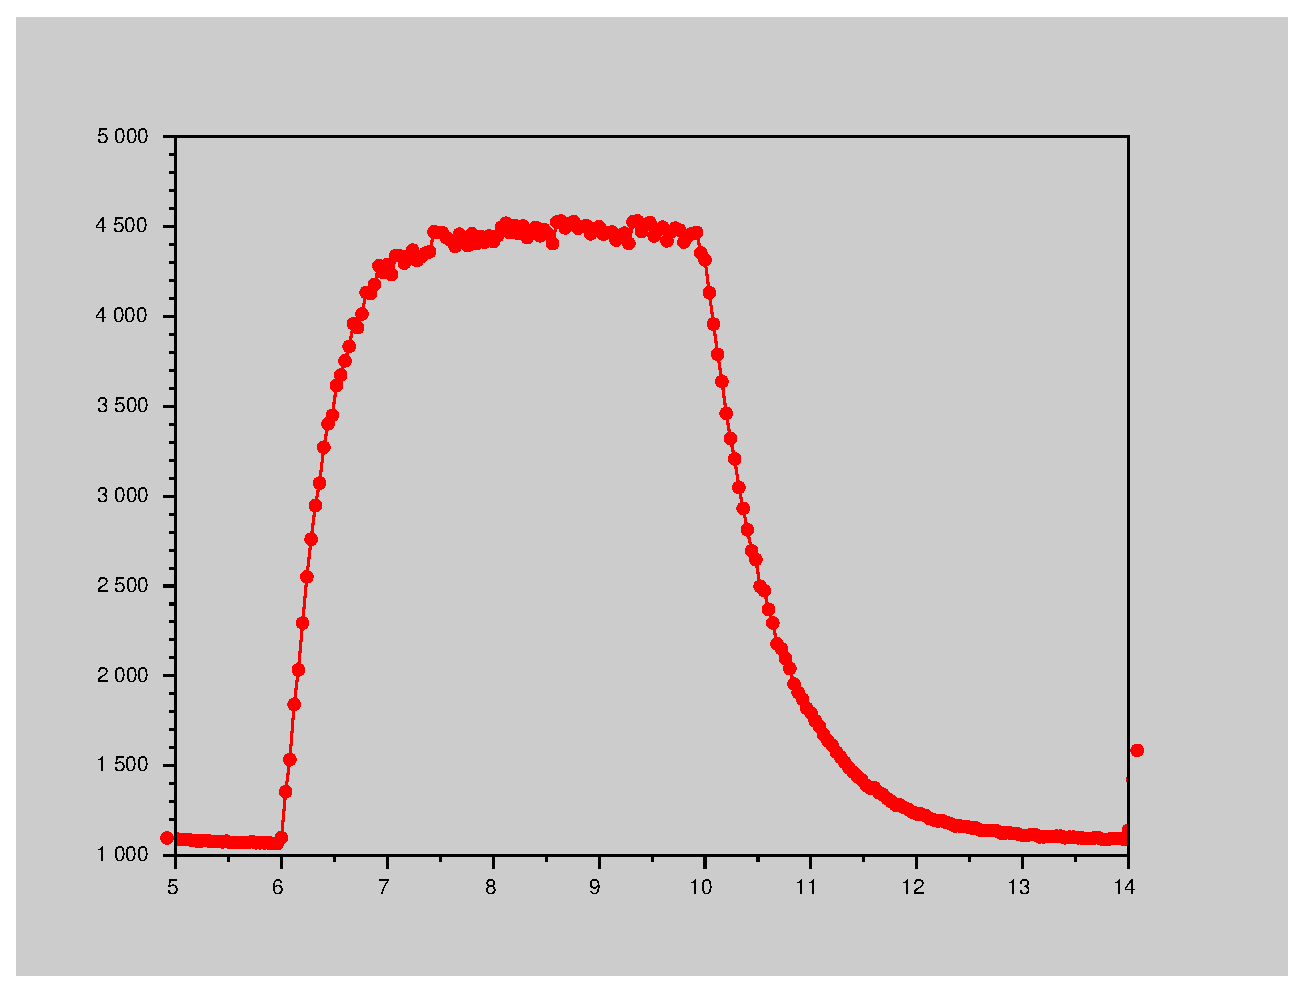
\includegraphics[width=7.0cm]{images/kadai5-1-3-expand.eps}
\caption{課題5.1拡大グラフ画像}
\label{fig:kadai5-1-3-expand}
\end{center}
\end{figure}

duty比に関しては

\begin{eqnarray}
duty比のhigh & = & 0.30 \\
duty比のlow &  = & 0.20 \\
duty比のステップ信号の高さ & = & 0.30 - 0.20 = 0.10
\end{eqnarray}

出力6秒から14秒の間を見ると

\begin{eqnarray}
出力のhigh & = & 4500 \\
出力のlow &  = & 1100 \\
ゲインK & = & \frac{3400}{0.10} = 34000
\end{eqnarray}
また時定数は
\begin{equation}
4500 \times 0.632  =  2844 
\end{equation}
より2844までの到達時間なので
\begin{equation}
T = 6.4 - 6 = 0.4
\end{equation}

\subsection{ステップ応答のシミュレーション}
求めた伝達関数のステップ応答をグラフに表示せよ. \\

以下図\ref{fig:kadai5-1-3-simu}に求めた伝達関数のステップ応答のグラフを示す.

\begin{figure}[H]
\begin{center}
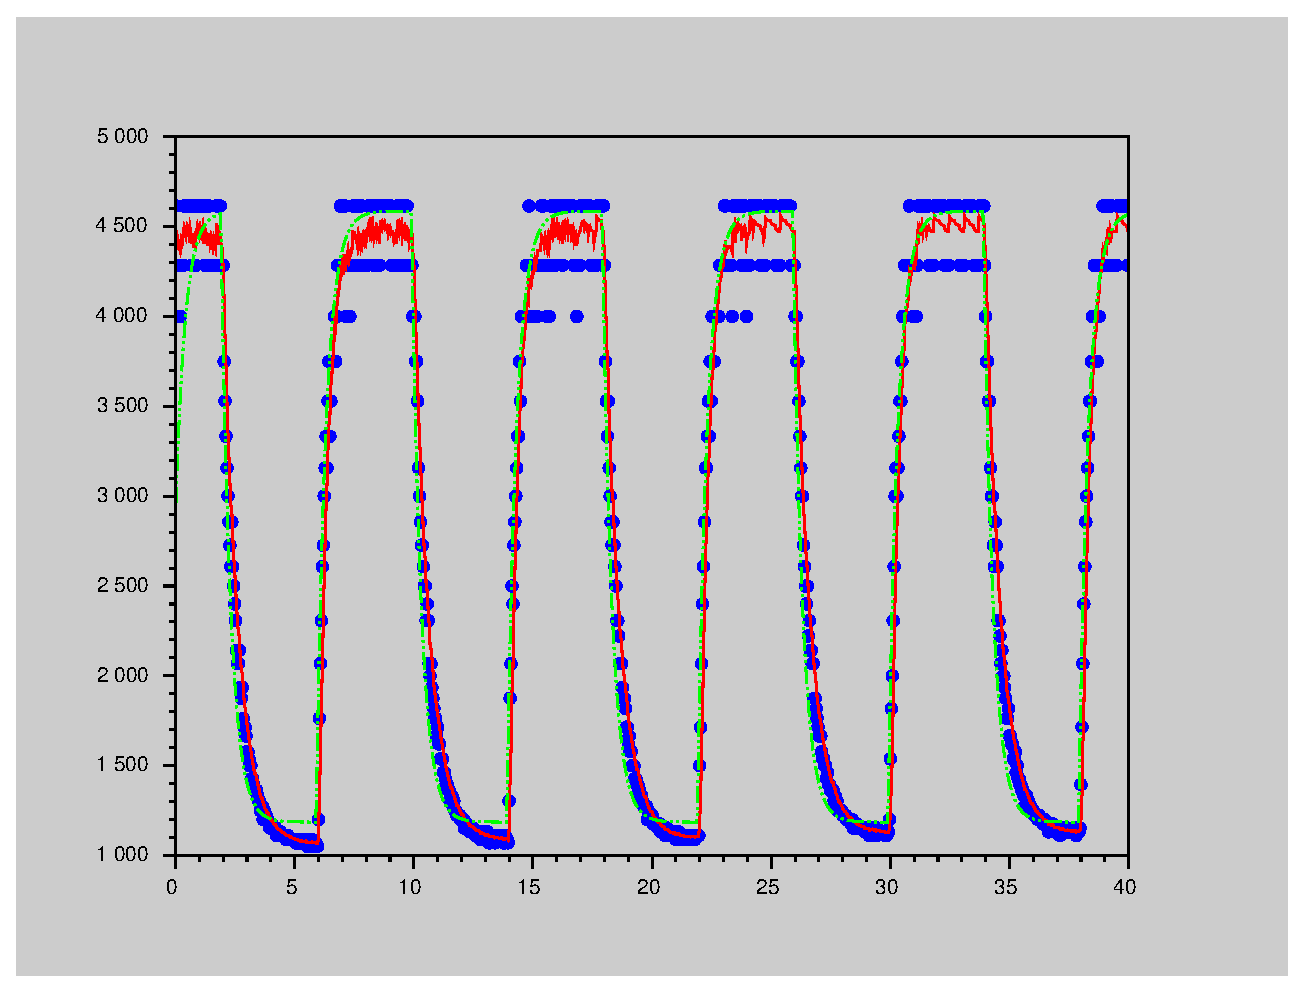
\includegraphics[width=7.0cm]{images/kadai5-1-3-simu.eps}
\caption{課題5.1ステップ応答}
\label{fig:kadai5-1-3-simu}
\end{center}
\end{figure}

\subsection{フィードバックゲイン}
求めた伝達関数をもとに,次回の課題6.1で使うフィードバックゲイン$K_P$,$K_I$を求めよ. \\

$\sigma= 0.5$として求めると
\begin{equation}
\frac{1 + 34000K_P}{34000K_I} = \sigma = 0.5
\end{equation}

\begin{equation}
\frac{0.5}{34000K_I} = 0.5\sigma^2 = 0.5 = 0.125
\end{equation}

より,
\begin{equation}
K_I = 0.00012 = 1.2 \times 10 ^{-4}
\end{equation}

\begin{equation}
K_P = 0.00003 = 3.0 \times 10 ^{-5}
\end{equation}
\section{LPFの時定数の影響}
\subsection{目的}
課題5.2の目的は何か?50字以上で答えよ. \\

課題5.2では$\alpha$の値を変えることでグラフにどのような影響が出るのか調べ,LPFの時定数が及ぼす効果について理解を深めた.ここで$\alpha$とはフィルタの出力の重みに相当するものであり,割り算の際の制度がなるべく落ちないように2のべき乗を選ぶことが多い.今回の実験では,2,4,8で行った.


\subsection{実験結果}
課題5.2の結果を報告せよ.その際,モータの回転速度,duty比などのデータをScilabを用いてグラフにすること. \\

以下図\ref{fig:kadai5-2-1-1}にモータの回転速度とと時間のグラフを示す.

\begin{figure}[H]
\begin{center}
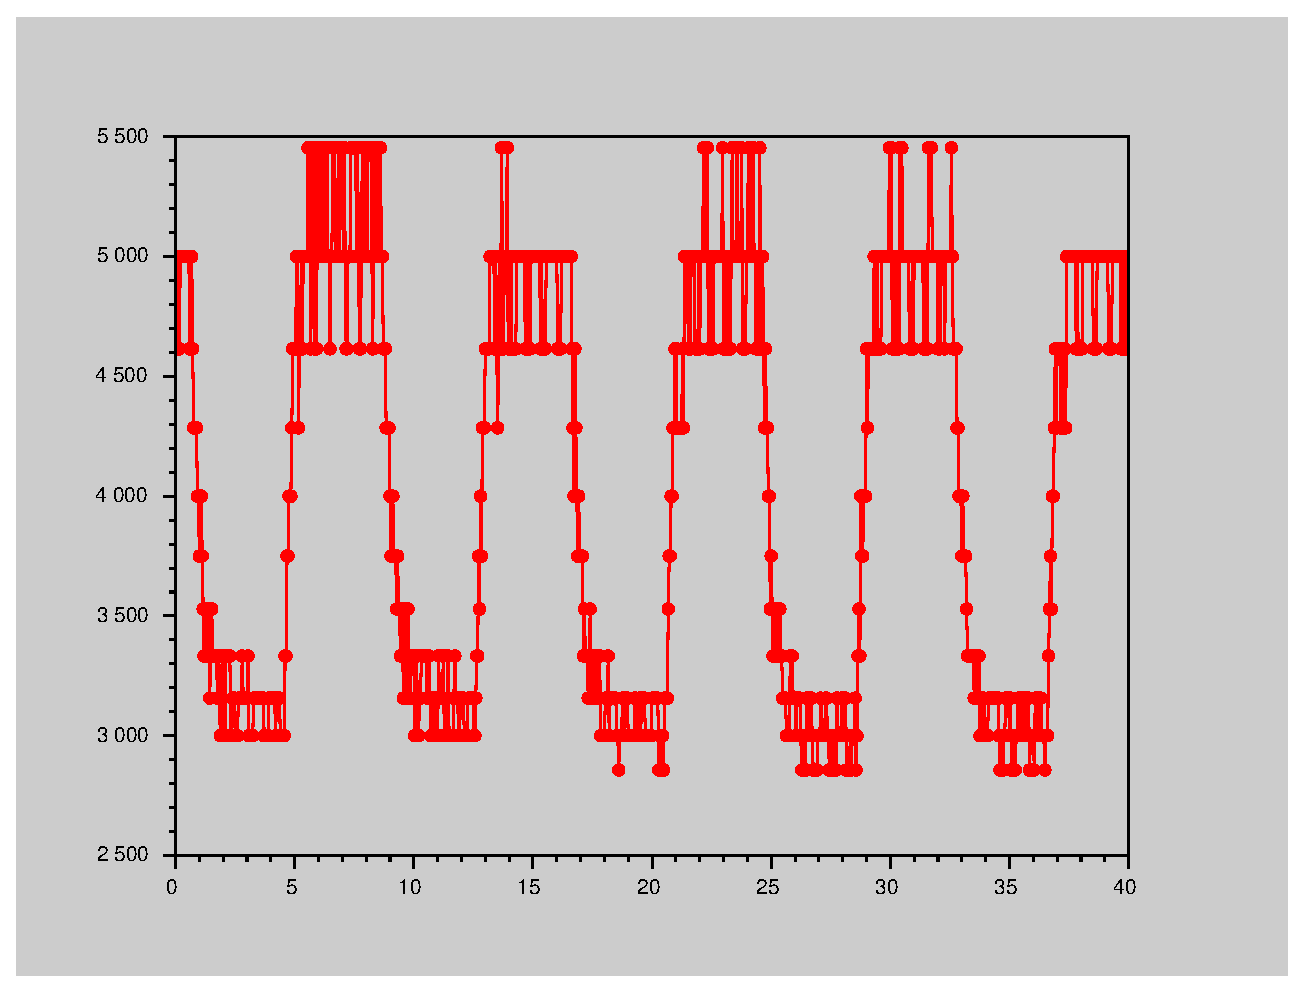
\includegraphics[width=7.0cm]{images/kadai5-2-1-1.eps}
\caption{課題5.2の出力画像(平滑化なし)}
\label{fig:kadai5-2-1-1}
\end{center}
\end{figure}


以下図\ref{fig:kadai5-2-1-2}にduty比と時間のグラフを示す.

\begin{figure}[H]
\begin{center}
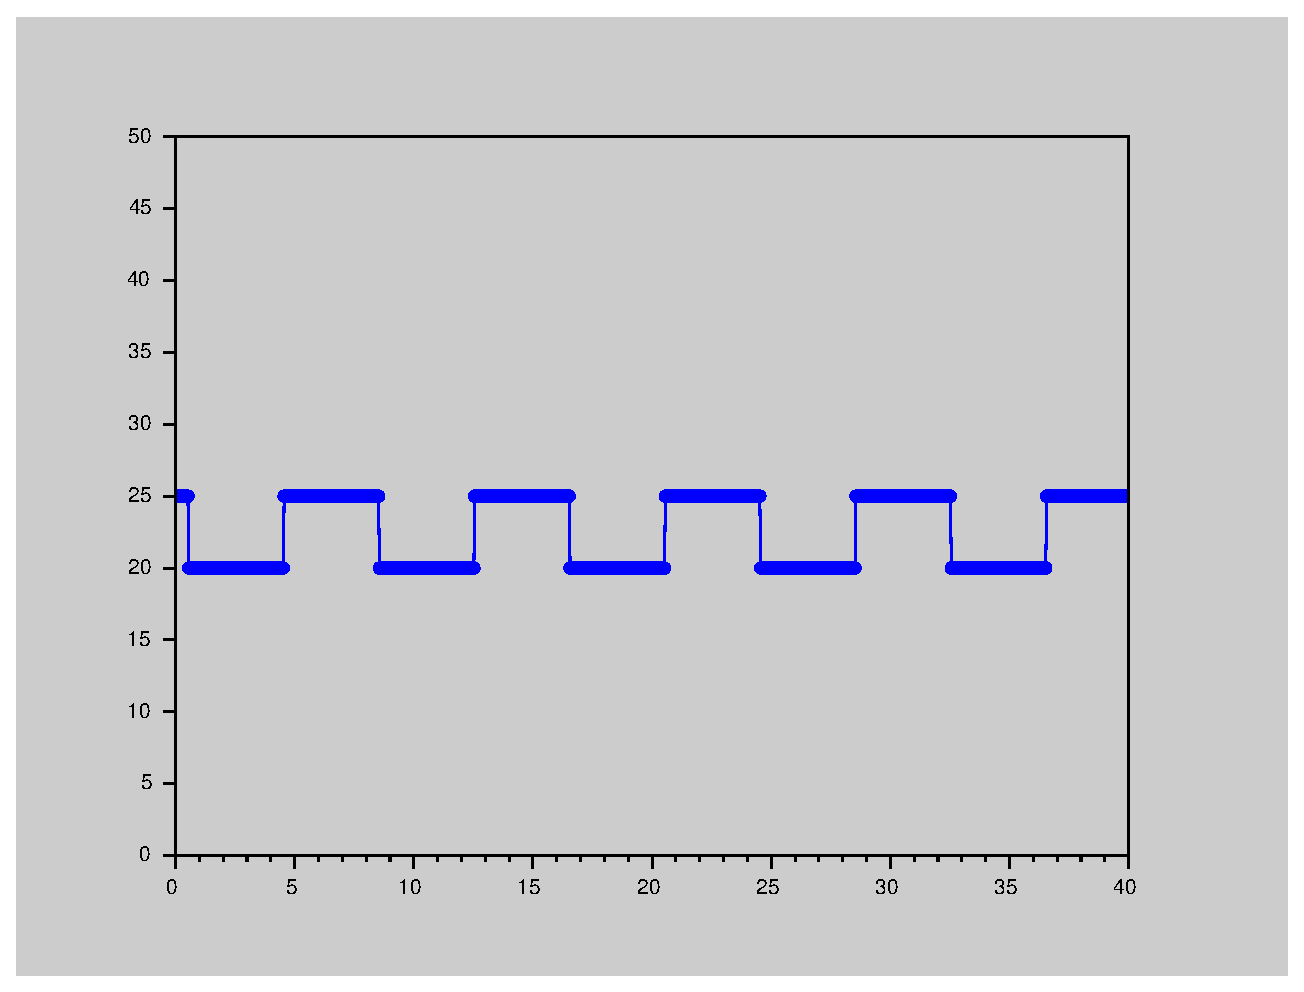
\includegraphics[width=7.0cm]{images/kadai5-2-1-2.eps}
\caption{課題5.2の出力画像(duty比)}
\label{fig:kadai5-2-1-2}
\end{center}
\end{figure}


以下図\ref{fig:kadai5-2-1-3}に$\alpha=2$のLPFを通し平滑化した後のモータの回転速度と時間のグラフを示す.

\begin{figure}[H]
\begin{center}
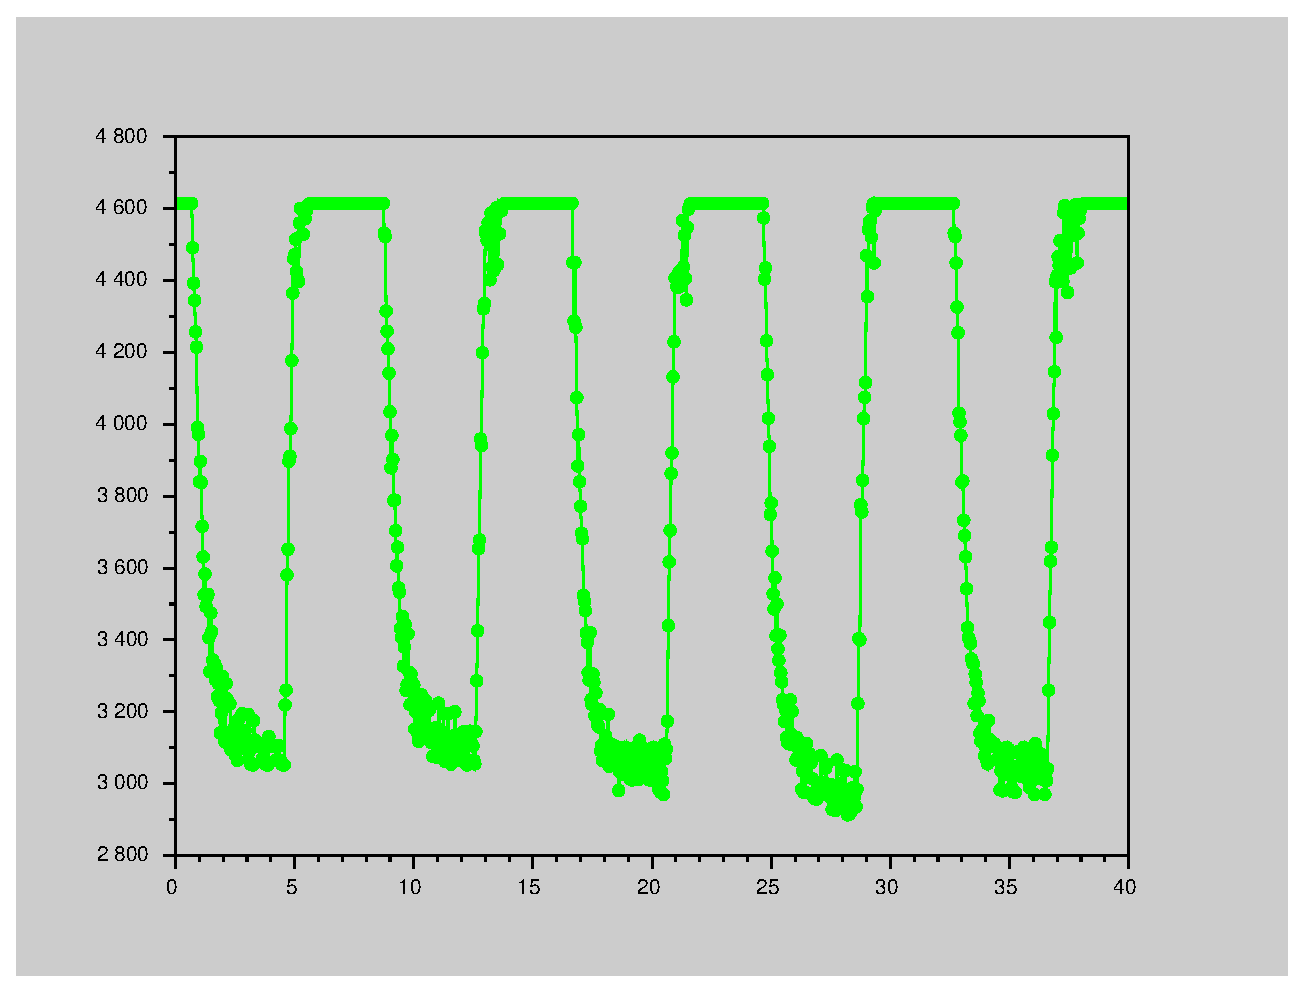
\includegraphics[width=7.0cm]{images/kadai5-2-1-3.eps}
\caption{課題5.2の出力画像($\alpha=2$)}
\label{fig:kadai5-2-1-3}
\end{center}
\end{figure}

以下図\ref{fig:kadai5-2-2-3}に$\alpha=4$のLPFを通し平滑化した後のモータの回転速度と時間のグラフを示す.

\begin{figure}[H]
\begin{center}
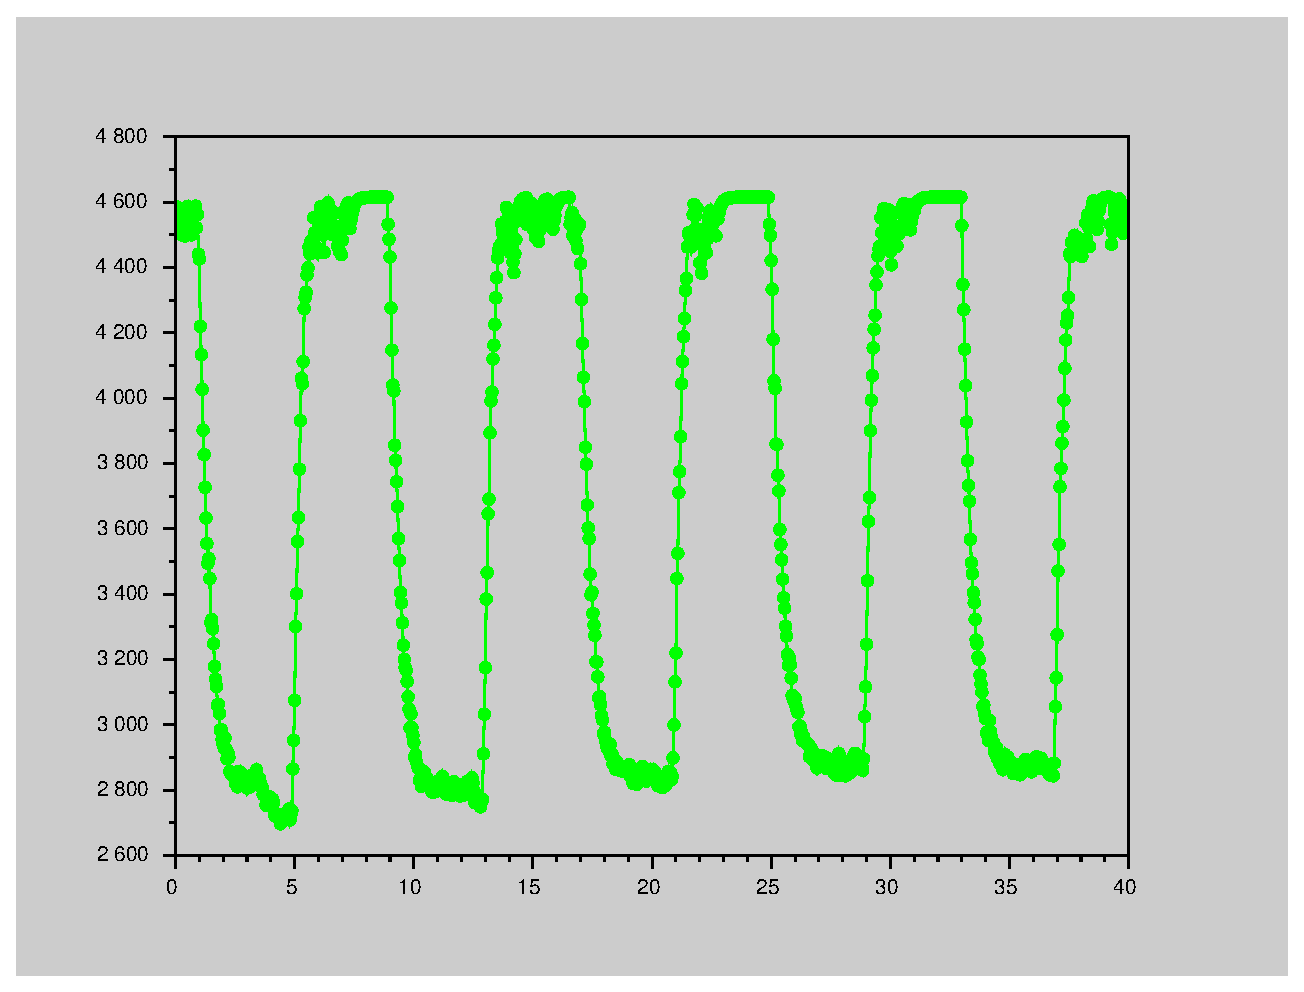
\includegraphics[width=7.0cm]{images/kadai5-2-2-3.eps}
\caption{課題5.2の出力画像($\alpha=4$)}
\label{fig:kadai5-2-2-3}
\end{center}
\end{figure}


以下図\ref{fig:kadai5-2-3-3}に$\alpha=8$のLPFを通し平滑化した後のモータの回転速度と時間のグラフを示す.

\begin{figure}[H]
\begin{center}
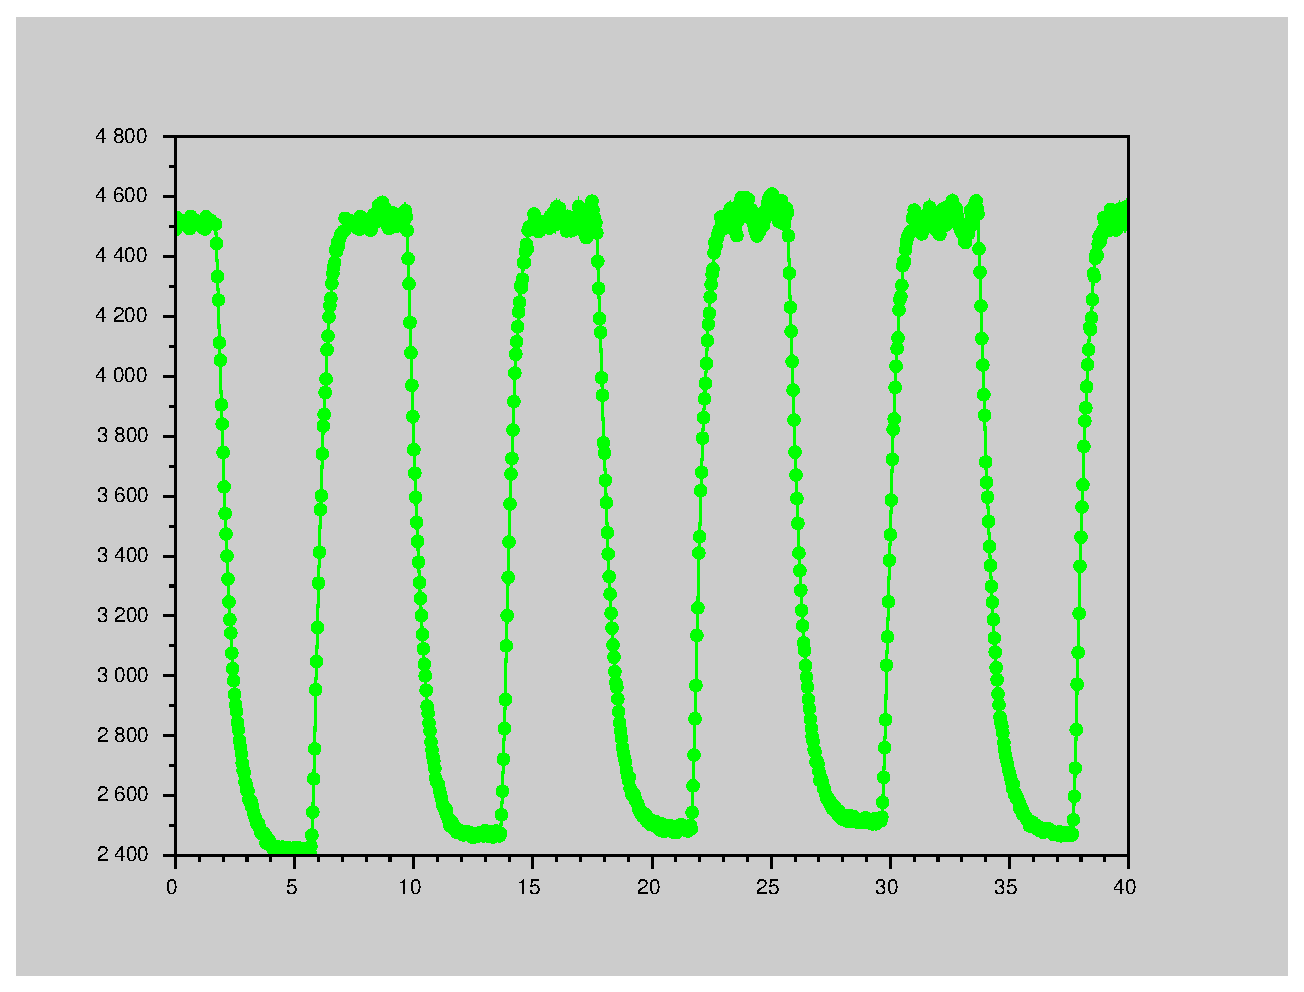
\includegraphics[width=7.0cm]{images/kadai5-2-3-3.eps}
\caption{課題5.2の出力画像($\alpha=8$)}
\label{fig:kadai5-2-3-3}
\end{center}
\end{figure}

\subsection{時定数の影響}
$\alpha=2,4,8$の場合で,立ち上がりの際の遅れや,定常状態における雑音の影響などを比較せよ.必要ならば拡大したグラフを作成せよ.

図\ref{fig:kadai5-2-1-3}と図\ref{fig:kadai5-2-3-3}を見比べると,$\alpha$の値が大きくなると立ち上がりに遅れが生じているのがわかる.また,$\alpha$の値が大きくなると定常状態における雑音の影響は小さくなり,比較的きれいなグラフになっている.

\end{document}





